\documentclass[12pt]{ctexart}
% set the left/right margin such that the main title can be written within one line
\usepackage[left=30mm]{geometry}
\usepackage{enumitem}
\AddEnumerateCounter{\chinese}{\chinese}{}
\usepackage{fancyhdr}
\usepackage{graphicx}
\usepackage{amssymb}
\usepackage{longtable}
\usepackage{hyperref}
\usepackage{subcaption}
\fancypagestyle{runningpage}
{
  \fancyhead{}
    \fancyhead[L]{
\includegraphics[height=18pt]{zijing_transparent.png}} 
    \fancyhead[C]{清华大学深圳研究生院紫荆志愿团}
  \fancyfoot{}
  \fancyfoot[C]{第 \thepage 页}
}
% not works?
\ctexset {
 appendixname = {附录}
}
\def\CurriculumScheduleWidth{1.6cm}
\begin{document}
% first page is cover
\title{
    \vspace{-0.5in}
    \textmd{\textbf{\huge{2019寒假清华深研院紫荆志愿团 \\ 爱心支教}}}\\
    \normalsize\vspace{0.1in}\Large{2018年秋季学期}\\
    \vspace{1in}
     \textbf{\huge{策}}\\
    \vspace{1in}
     \textbf{\huge{划}}\\
    \vspace{1in}
     \textbf{\huge{书}}\\
    \vspace{1in}
}
\author{策划人:赵丰、张晓冰}
\maketitle
\thispagestyle{empty}
\pagebreak
\pagestyle{runningpage}
\tableofcontents
% 为什么要联合5所高校?
% 实际:方便拉赞助
% ideal: 规模效应,影响力。

% 有没有能力组织,可行性如何?
% 退一万步说:即使没拉到赞助,志愿者车费全部自费也是比较吸引人的。毕竟其他支教队好多都无法报销车费的。有的,高校义工之间合作比较频繁。

% 能不能拿到官方支持?
% 难说。有利的一面是只是口头支持,不用官方掏钱。但既然官方出面,深圳这边媒体报道必须少不了。
% 不利的一面,人太多,不安全?
% 破:强调是一个松散的联盟。实际还是各高校自行组织。强调时代大背景:教育扶贫。深圳慈展会刚开完。

% 突破点:大公司的支持。腾讯公益啥的稍微支持一下就能把4万多的车费(60人)解决掉。
% 当地官方的支持也很重要。

% 短期支教弊端怎么破?
% 强调科学启蒙、寒假夏令营。

\section{项目背景}
清华大学致力于培养科研与德育全面发展的高素质人才,清华大学深圳研究生院紫荆志愿者团作为院团委的直属组织,始终坚持先进青年助人为乐、奉献社会的精神,是一支优秀的志愿团队。志愿团的成员不仅积极参与院内外的各类志愿活动,还负责与相关部门对接,招募志愿者,组织、协调活动。

%除了大学城三所高校外,在片区内还坐落着南方科技大学、中国科学院先进技术研究院以及深圳大学西丽校区。美丽的大沙河横穿六所高校校区。2018年秋季学期,通过深圳高校大型节水志愿活动、2018中国开源年会志愿服务以及南山区半程马拉松志愿服务等活动,六所高校的志愿组织密切协作,共同完成志愿者的招募和培训,活动的开展以及后期宣传等。
%本次联合支教即为六所高校志愿组织协商后一致同意的志愿项目。

党的“十九大”以来,基层的脱贫攻坚作为基层工作的重点在全国推行。习总书记曾提出,“扶贫必扶智”。海南省琼海市嘉积镇是国家重点扶贫单位。作为清华深研院的学子,我们希望能开拓志愿服务的思路,响应基层扶贫的号召,利用寒假社会实践的机会,以“教育扶贫”为主题,深入当地开展支教活动。

海南省“美在心灵”大学生支教志愿者协会在寒暑假与高校团队对接、共同组织开展在海南的支教活动由来以久。
本次支教即选择在海南省琼海市并与美在心灵琼海分会密切合作。我们希望在本次支教活动中可以进一步深入调研当地基础教育的建设情况,形成有价值的调研报告,在为当地基层教育事业作出切实贡献的同时,也能够为当地基础教育的长远发展提供参考。

\section{项目目标}
\begin{itemize}
\item 本院:扩大志愿团志愿服务的范围,进一步宣传院团委等。
\item 参与者:体验短期支教生活,培养吃苦耐劳、乐于奉献的精神,形成对科研生活的有益补充。
\item 支教地:提升支教地重视少年STEM教育的氛围,为当地基础教育的发展作出切实贡献。
\item 支教学生:打开孩子的视野,促进孩子的心灵成长。
\end{itemize}
\section{项目简介}
\begin{itemize}
\item 主办方:清华大学深圳研究生院紫荆志愿者团
\item 协办方:美在心灵大学生支教志愿者协会
\item 地点:海南省琼海市嘉积镇长江学校(初中)
\item 时间:2019年1月XX日至2019年1月XX日,在支教地一周
\item 志愿者: 清华深研院在校生
\section{项目特色}
随着人工智能的发展,编程作为技术手段之一地位逐渐突出。2017年国务院《新一代人工智能发展规划》指出在中小学
“推广编程教育,鼓励社会力量参与”。

传统的益智积木在电子信息技术的发展影响之下也趋向于“机电一体化”,作为一种高级玩具,在诸如深圳这种一线城市,每年均会针对中小学生举办机器人设计大赛。但相比之下,很多贫困地区的孩子并没有机会接触这些。为了弥补这一缺憾,紫荆团队打算继续与搭搭乐乐合作,筹集善款,以成本价购买机器人套装作为寒假支教教具,并在支教结束后无偿捐献给支教学校。

2018年暑假,北航在美丽中国的赞助下赴云南给大理巍山县的两所中小学开展了为期一周的科技夏令营,所需器材由美丽中国出面获得萝卜太辣公司的赞助;无独有偶,在深圳这座科技创新之城,清华深研院紫荆志愿团获得搭搭乐乐的赞助与海南美在心灵合作赴海南儋州开展科技夏令营。

2019年寒假,紫荆志愿团队希望在暑假活动基础上将“科技支教”作为寒暑假一个长期的项目运营,尽团队微薄之力给乡村的孩子带去STEM启蒙。作为云集了全国机械、电子领域最优秀的研究生的科研院所,紫荆志愿团队必将能圆满完成项目目标。
%\begin{table}[!ht]
%\centering
%\begin{tabular}{|c|c|c|c|c|}
%\hline
%姓名 & 性别 & 年级 & 系别 & 联系方式\\
%\hline
%赵丰 & 男 & 研一 & 电子系 & 18800190762 \\
%\hline
%张晓冰  &	男	& 研一 &  生物系 & 13938315159 \\
%\hline
%张炎武 & 男 & 研一 & 医院管理 & 18894000752\\
%\hline
%白杨 & 女 & 研一 & 电子系 & 18810913823\\
%\hline
%王鲜俐 & 女 & 研一 & 材料系 & 17633905356\\
%\hline
%黄少平 & 男 & 研一 & 自动化系 & 13696922357\\
%\hline
%周俞君(琼) & 女 & 大一 & 学前教育 & 13036084399 \\
%\hline
%周让强(琼) & 女 & 大二 & 医药营销 & 13518025473 \\
%\hline
%\end{tabular}
%\caption{参与支教志愿者名单}
%\end{table}
\end{itemize}
\section{项目实施方案}
\begin{enumerate}
\item 筹集支教物资
\item 与校长沟通,确定食宿方案
\item 【可选】寻求商家的赞助
\item 招募志愿者
\item 志愿者准备教案
\item 志愿者行前碰面会两次
\item 志愿者部分统一购买车票、出行保险
\end{enumerate}


\section{项目流程}
\begin{table}[!ht]
\centering
\begin{tabular}{|c|c|}
\hline
时间 & 安排 \\
\hline
 &  从深圳出发,经广州抵达海口、从海口 \\
\hline
 & 从海口乘动车抵达琼海站,转大巴到长江学校\\
\hline
 & 开营仪式\\
\hline
 & 日常支教活动,穿插家访、调研 \\
\hline
 & 结营仪式 \\
\hline
 & 志愿者返回 \\
\hline
\end{tabular}
\caption{行程安排表}\label{route}
\end{table}



\section{项目后续阶段}
\begin{enumerate}
\item 整理资料,提交实践材料;完成往返火车票部分报销、出行保险报销;参与答辩等。
\item 借鉴“旧洋关爱组”,对支教地的孩子给予持续的成长关注。
\end{enumerate}
\section{联系方式}
清华大学深圳研究生院紫荆志愿者团:赵丰

Tel: 18800190762

Email: 616545598@qq.com

\begin{flushright}
\the\year 年 \the\month 月 \the\day 日
\end{flushright}

\begin{appendix}

\section{关于清华大学深圳研究生院紫荆志愿者团}
清华大学深圳研究生院紫荆志愿者服务团是清华大学深圳研究生院团委直属的学生志愿服务组织,以“自我实践、服务他人、自我教育、推动社会”为宗旨,旨在组织、协调我院研究生志愿者活动,开展具有清华特色的丰富多彩的研究生志愿活动。
\begin{figure}[!ht]
\centering
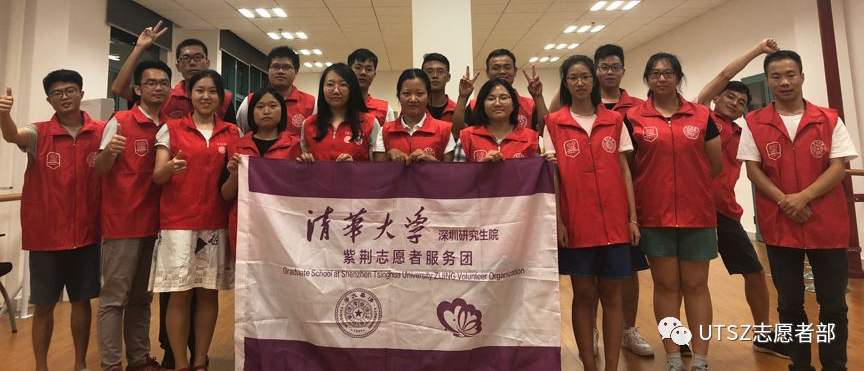
\includegraphics[width=14cm]{pic/zijing.png}
\end{figure}
2018年暑假,紫荆志愿团在海南省儋州市开展了支教扶贫系列活动,开拓了高校团队机器人支教的先河。


本次寒假清华大学深圳研究生院紫荆志愿者团拟开展的支教活动希望以成本价购入儿童机器人套装作为教具,发挥
自身专业优势开展支教活动。通过研究生寒假社会实践体系实现车费的报销。
%\begin{table}[!ht]
%\centering
%\begin{tabular}{|p{2cm}|p{2cm}|p{2cm}|p{3cm}|}
%\hline
%名称 & 来源 & 用途 \\
%\hline
%%深圳市搭搭乐乐文化传播有限公司
%儿童、初中机器人套装&  &  \\
%\hline
%素质拓展道具 & 心理辅导中心 &  \\
%\hline
%DOBOT魔术师(价值一万元) & 越疆科技 & \\
%\hline
%教具& &  \\
%\hline
%文具奖品 & & 课堂奖励 \\
%\hline
%\end{tabular}
%\caption{清华支教队所需教具参考}
%\end{table}

关于“旧洋关爱组”:旧洋村是一个支教点,紫荆团队和琼台师范学院2018年暑期在此支教。旧洋关爱组的实体是一个QQ群,由紫荆团队、琼台师范学院和支教地的孩子组成。各位支教老师利用自己的业余时间针对孩子暴露出的问题进行有针对性的疏导。紫荆团队在中秋佳节专程到东莞看望支教点的一个辍学的孩子,他现在跟着父母在莞城打工。
\begin{figure}[!ht]
\centering
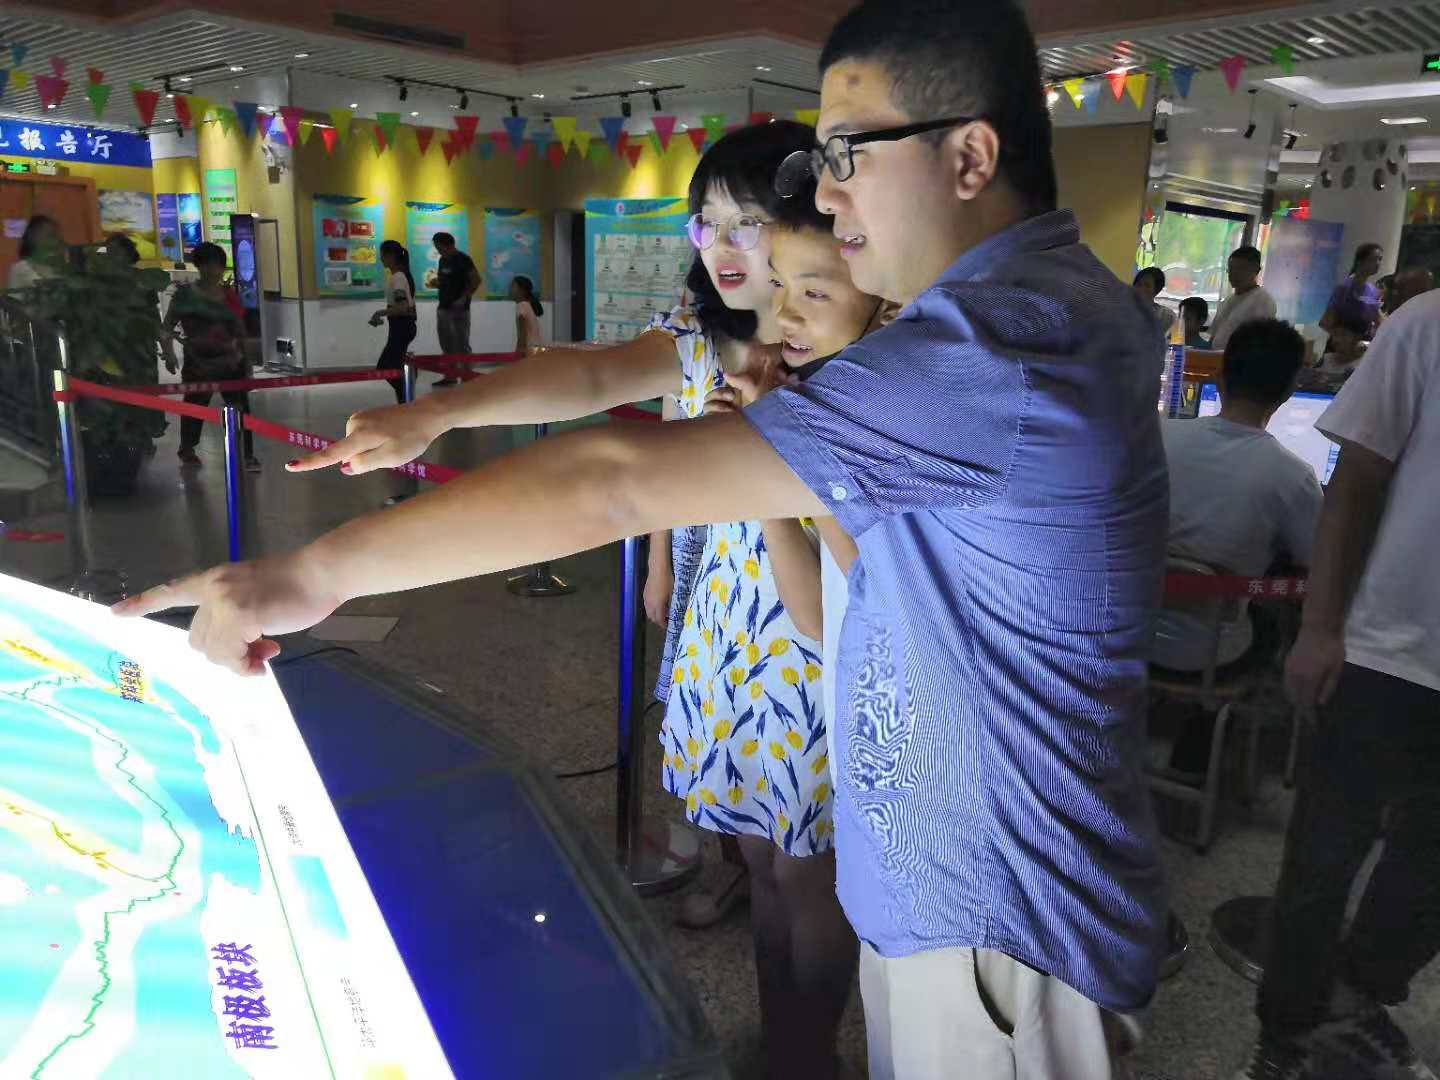
\includegraphics[width=12cm]{pic/zijing_talk.jpeg}
\caption{紫荆志愿者在东莞科技馆给孩子讲解}
\end{figure}
\section{关于美在心灵}
海南省“美在心灵”大学生支教志愿者协会(简称美在心灵)于2008年1月30日诞生于琼海市嘉积中学,2010年3月29日接受共青团海南省委业务主管,2011年7月11日在海南省民政厅注册成为合法民间公益机构,2017年12月6日被海南省民政厅授予“慈善组织”资格。美在心灵以“团结友爱,奉献社会”为宗旨,不以盈利为目的,广泛招募世界各地大学生志愿者到琼藏等乡村小学开展爱心支教活动,致力给孩子们一个快乐成长平台,给大学生一个社会实践机会,给社会一个务实且放心的爱心渠道,给政府一个温暖的辅助。目前已有美国、英国、俄罗斯、新加坡、韩国、日本等40多个国籍的大学生志愿者,以及清华、北大、港澳台等境内国内名校的大学生志愿者参加支教活动。十年以来,美在心灵安排志愿者1.9万人次,服务小学754所次(包括西藏两所小学:恩达小学和宾达小学),受益学生6.2万人次,总服务时长165万小时,总投入善款158万元。

\section{项目财务预算}\label{scheduling}
%所需物资具体到总共要多少钱


\begin{enumerate}
\item 往返车票:通过寒假实践流程可予以报销、部分需要由商家赞助或志愿者自费。单人单程350元左右。
\item 住宿费:由当地学校帮忙解决。由于购置生活必需品产生的开支单人单程50元左右。
\item 餐饮,部分由当地学校承担、部分由相关商家赞助费用、部分由志愿者自费。预估单人7天需要350元左右。
\item 教具(如机器人与科技产品等)与宣传资料:部分通过校团委报销、部分由相关文娱企业赞助。
\item 物资邮寄费用:部分由当地政府承担、部分需要由企业赞助。统一邮寄可节省开支,预估单程200元。
\item 志愿者出行保险:通过寒假实践流程可予以报销。单人7天需要20元左右。
\item 助学物资:商家赞助。
\end{enumerate}
按10人参与计算,不含教具和助学物资,预估总费用 12000元。
\section{关于自筹善款部分}
\begin{table}[!ht]
\centering
\begin{tabular}{|c|c|p{3cm}|p{2cm}|}
\hline
项目 & 额度 & 商家  & 总费用 \\
\hline
初中机器人套装 &  10套 & 深圳市搭搭乐乐文化传播有限公司 & 4000(成本价+含邮寄费) \\
\hline
书籍 & 若干 &  当当图书网 & 600 \\
\hline
文具和小奖品、清华纪念品 & 若干 & 西丽文具店 & 400 \\
\hline
\end{tabular}
\caption{教具}
\end{table}
以上所有购买的教具总额度为5000元以内,希望通过社会爱心企业赞助或其他大赛奖励获得。支教结束后所有教具均捐献给支教学校。物资的捐赠特别是机器人支教方面物资的捐赠使得对方学校从无到有初步具备起机器人课程所需的器材。
\section{赞助方案}
我们为赞助商设计了不同的合作方案以满足您多样化的需求。根据赞助金额的不同,我们初步设计了如下三个档位的赞助方案:
\begin{itemize}
\item 方案A——赞助4000元;
\item 方案B——赞助2000元; 
\item 方案C——赞助1000元。
\end{itemize}
不同赞助档位享受的宣传回报(见下表)有所不同,您可以根据自己的预算与想要实现的宣传力度选择合适的档位,如果这些都不能满足您的需要,具体的赞助金额以及赞助回报还可结合您的具体情况最终决定。目前初步拟定的赞助回报具体实施方案如下:
\begin{table}[!ht]
\centering
\begin{tabular}{|c|c|c|c|}
\hline
赞助方案 & 方案A & 方案B & 方案C \\
\hline
活动宣传 & \checkmark & \checkmark & \checkmark \\
\hline
现场鸣谢 & \checkmark &  \checkmark & \\
\hline
公众号文章宣传与转载 & \checkmark & &\\
\hline
活动冠名 & \checkmark & & \\
\hline
\end{tabular}
\end{table}

\begin{itemize}
\item 活动宣传:在各高校义工联公众号上的线上宣传中,均特殊标记鸣谢活动赞助商。
\item 现场鸣谢:在开营、闭营活动中,主持人鸣谢活动赞助商的大力支持。
\item 公众号文章宣传与转载:由支教队提供突出赞助商的文章,可由赞助商公众号进行转载。
\item 活动冠名:冠名赞助商以承办方。
\end{itemize}
备注:除了三种方案,我们欢迎有兴趣的商家赞助文具,高档食品等。如果商家有其他赞助需求,可以进一步商谈,定制方案。


\section{志愿者保障和守则}
\subsection{保障}
\begin{enumerate}
\item 志愿深圳平台工时。
\item 志愿者出行人身意外保险。
\item 住宿保障。
\item 一定额度的往返车费补贴和餐饮补贴。
\end{enumerate}
\subsection{守则}
\begin{enumerate}[label = {(\chinese*)}]
\item 具有完全民事行为能力的学生;
\item 认同紫荆志愿团理念和文化,尊重“美在心灵”的支教理念;
\item 服从支队长、村书记和相关爱心人士在支教期间的引导;
\item 有社会责任感和奉献精神,无不良嗜好;
\item 有较强的团结协作能力、语言表达能力和人际交往能力,尊重队友;
\item 有较强的心理素质,在艰苦的环境下能自我调节,保持积极乐观心态,肯吃苦,能坚持,不给支教项目及队友带来负面影响; 
\item 有爱心,热心帮助当地的学生和村民,尊重当地的民族文化和信仰;
\end{enumerate}
\end{appendix}
\end{document}

